\documentclass[sigconf,nonacm]{acmart}
\settopmatter{printacmref=false,printccs=false}
\renewcommand\footnotetextcopyrightpermission[1]{}
\pagestyle{plain}
\usepackage{amsmath}
\usepackage{graphicx}
\usepackage{booktabs}
\setlength{\emergencystretch}{3em}
\title{Native-Resolution Solar Filament Segmentation with Annotation-Aware Ensembles and Instance Rescoring}
\author{Shengkai Zhu}
\affiliation{\institution{Independent researcher}\country{}}
\renewcommand{\shortauthors}{Shengkai Zhu}
\begin{document}
\begin{abstract}
We describe the ens5c submission to the Solar Filament Segmentation Challenge
2026. The system combines five U-Nets with pretrained ResNet50 and ConvNeXt-S
encoders, native-resolution training crops, multiple-annotator supervision,
contact-aware instance formation, and a gradient-boosting instance rescorer.
The accepted submissions achieve public leaderboard Panoptic Quality (PQ)
0.40. The selected match-probability rescorer obtains local PQ 0.47404 under
observation-grouped nested rescorer evaluation, compared with 0.47236 for an
expected-IoU alternative. This difference is not statistically conclusive.
These local estimates are exploratory: the segmenters, ensemble, and
post-processing were previously selected using the same development split.
Experiments with detector candidates, additional test-time augmentation,
larger crops, and selective contour refinement motivate retaining the simpler
validated ensemble. The reproduction package includes exact checkpoint
bytes, configurations, inference code, two reference prediction files,
and checks for nonempty, nonoverlapping COCO RLE masks.
\end{abstract}
\keywords{solar filaments, instance segmentation, annotation disagreement, ensemble, panoptic quality}
\maketitle

\section{Task and design priorities}
The challenge requires one instance mask per solar filament in full-disk
GONG H-alpha observations. Each input is a $2048\times2048$ grayscale JPEG.
Filaments occupy a small fraction of the solar disk and can include narrow
barbs, interrupted dark segments, and nearby structures with similar
appearance. A semantic foreground prediction alone does not resolve which
pixels belong to the same physical object. In addition, annotations are
not a unique deterministic target: different observers can disagree about
object presence, boundaries, and grouping.

The official competition metric evaluates predictions against each
annotator record and pools the matching counts. Our main priorities are
therefore to preserve native image detail, keep all annotations of one
observation in the same data split, and evaluate the final instance pipeline.
A better pixel loss or an intermediate mask score is not sufficient evidence
of a better final submission. We use a modular approach: foreground and
contact prediction, instance formation, and learned instance filtering.
The contribution is an evaluated competition pipeline and its diagnostic
evidence, rather than a new segmentation architecture.

\section{Data and evaluation protocol}
The official training data contain 707 distinct observations with 1,154
annotation records. The test set contains 180 observations. An observation
can have up to three independent annotation sets. We reserve 106 observations
for development and train the segmenters on 601, stratifying the split by
observatory. Splitting by annotation ID would leak the same image across
partitions; our split operates on the original image filename. The exact
observation IDs are included in the package.

Training polygons are rasterized with pycocotools. Images and annotation
label maps are cached as NumPy arrays, and crops are accessed with memory
mapping. Annotation records remain separate for scoring. We do not access
the public MAGFiLO annotation release for competition test images, and no
test labels, external ground-truth metadata, or precomputed third-party
submission are used. Pretrained visual encoders supply generic image
representations; all task-specific segmentation supervision comes from the
permitted competition training split.

For the competition evaluator, a true-positive match requires strict
$\mathrm{IoU}>0.5$. The aggregate metric is
\begin{equation}
\mathrm{PQ}=\frac{\sum_{(g,p)\in\mathrm{TP}}\mathrm{IoU}(g,p)}
{|\mathrm{TP}|+\tfrac12|\mathrm{FP}|+\tfrac12|\mathrm{FN}|}.
\end{equation}
We sum numerators and counts across annotation records, rather than
averaging per-image PQ. The public score is rounded and is computed on
only part of the test set; it is not interchangeable with local development
PQ. The local rasterized instance maps can overwrite rare overlapping
ground-truth polygons. A separate overlap audit exists in the research code;
this representation is an additional limitation of local comparisons.

\section{System overview}
Five models predict foreground and inter-instance contact probabilities.
Four flip orientations are inverted and averaged for each model; model
probabilities are then averaged with equal weights. A foreground threshold
and contact-aware watershed create candidates, nearby fragments can be
merged, and a learned regressor filters candidates. A single label map
guarantees that the output masks of one image are disjoint. The same
segmentation maps support the match-probability and expected-IoU final
rescorers. Their difference lies in the learned scoring target, not the
five segmentation checkpoints.

\clearpage
\section{Segmentation models and training}
\subsection{Architecture and initialization}
Each model uses a U-Net decoder~\cite{unet}, with either a ResNet50
encoder~\cite{resnet} initialized from ImageNet or a ConvNeXt-S
encoder~\cite{convnext} initialized with DINOv3 weights~\cite{dinov3} through
\texttt{timm}. ConvNeXt remains a convolutional architecture even when using
DINOv3 pretraining. The selected submission does not contain a vision
transformer. The SMP implementation adapts the first convolution to one
input channel; we do not treat the solar images as color observations.
Intensities are scaled to $[0,1]$ and normalized as $(x-0.45)/0.225$.
The two output logits represent foreground and contact regions.

\begin{table}[h]
\caption{The five selected checkpoints. ``Random'' chooses one annotator
per crop; ``consensus'' uses the fraction marking each pixel.}
\centering\small
\begin{tabular}{llll}
\toprule
Run & Encoder & Target & Step\\
\midrule
r50-long & ResNet50 & Random & 21,000\\
cnx-s-bce & ConvNeXt-S & Random & 10,500\\
cnx-s-long & ConvNeXt-S & Random & 28,500\\
r50-consensus & ResNet50 & Consensus & 21,000\\
cnx-s-consensus & ConvNeXt-S & Consensus & 21,000\\
\bottomrule
\end{tabular}
\end{table}

\subsection{Sampling and augmentation}
We train on $512\times512$ crops without resizing the original image.
With probability 0.8, a crop is centered near a randomly chosen filament
centroid, with a Gaussian center perturbation. Otherwise it is sampled
within the solar disk. Each sampling event selects an observation and
an anchor annotator. This prevents observations with more annotation sets
from automatically dominating the sampling distribution.

The generator extracts extra context before geometric augmentation.
It applies a continuous random rotation in $[0,360)$ degrees, scaling in
$[0.85,1.15]$, and a horizontal flip with probability 0.5. The identical
geometric transformation is applied to the image and every annotation map;
images use linear interpolation, labels nearest-neighbor interpolation.
Photometric augmentation multiplies intensity by a factor in $[0.8,1.2]$,
adds an offset in $[-0.08,0.08]$, and applies a gamma in $[0.7,1.4]$.
Gaussian blur and additive Gaussian noise are each applied with probability
0.3. Intensities are clipped to the valid range. These transformations
simulate viewing orientation and image-quality variation without requiring
new labeled observations.

\subsection{Annotation targets and loss}
Random-annotator models use one binary foreground mask per crop. Consensus
models instead use the fraction of annotators marking a foreground pixel,
providing a soft target. This is an empirical way to expose disagreement,
not a claim that majority voting is the optimal rule for instance PQ.
The contact target marks pixels within a small neighborhood of two distinct
instances. We avoid marking every object contour as a separating boundary:
many thin filaments would be destroyed by removing their entire edge.
For consensus training, contact targets are combined across annotators.

The selected models optimize foreground binary cross-entropy plus Dice,
and a contact loss with weight 0.5:
\begin{equation}
\mathcal{L}=\mathcal{L}_{\mathrm{BCE,fg}}+\mathcal{L}_{\mathrm{Dice,fg}}
+0.5(\mathcal{L}_{\mathrm{BCE,contact}}+\mathcal{L}_{\mathrm{Dice,contact}}).
\end{equation}
Positive contact pixels receive BCE weight 5. Skeleton and focal-loss
experiments are not part of the selected checkpoint recipe.

\subsection{Optimization and checkpoint selection}
The runs use AdamW, decoder learning rate $3\times10^{-4}$, an encoder
rate ten times smaller, weight decay $10^{-4}$, batch size 8, mixed
precision, gradient clipping at norm 1, and a 300-step warmup. A plateau
schedule reduces learning rates when development PQ stalls. Exponential
moving-average weights use decay 0.999. Full-image development PQ selects
the saved checkpoints. Recorded per-run configurations and logs are the
authoritative source for the exact stopping trajectories. An interrupted
experiment retraining on all 707 observations is not used in the two
accepted submissions described here.

\section{Instance formation and learned filtering}
For the selected pipeline, foreground is thresholded at 0.5. Watershed
seeds exclude predicted contact pixels above 0.5. Components lacking a seed
are retained as separate candidates. Fragments belonging to different
connected components can be merged within 16 pixels. We evaluated simple
area/confidence thresholds, but the final pipeline replaces this last
filter with a learned instance rescorer.

The rescorer is a histogram gradient-boosting regressor with 300 iterations,
learning rate 0.04, at most 15 leaves, minimum leaf size 20, and L2
regularization 1. Features describe candidate geometry, predicted
probabilities, local contrast, solar-disk position, observatory, and year.
The primary target is the proportion of annotation records for which the
candidate matches an instance. The alternative averages matched IoU,
assigning zero for an unmatched annotator record. A scalar threshold decides
which candidates to retain, with the highest-scored candidate retained when
needed to maintain the submission coverage policy.

\clearpage
\section{Results and candidate selection}
\subsection{Public progression and local evidence}
The initial ResNet34 U-Net scored 0.35 on the public leaderboard. ResNet50
increased this to 0.37, and learned instance rescoring increased it to 0.38.
Longer training with EMA reached 0.39. Combining ResNet and ConvNeXt
representations with an expected-IoU rescorer reached 0.40. Later ensembles
improved local measurements but remained at the displayed public score 0.40.
The final two accepted ens5c files were resubmitted on 4 October 2026:
submission 56835266 uses the match target, and 56835269 uses expected IoU.

\begin{table}[h]
\caption{Selected local comparisons. Nested evaluation concerns the
rescorer, not independent selection of the entire pipeline.}
\centering\small
\begin{tabular}{lrr}
\toprule
Pipeline / rescorer & Local PQ & Public PQ\\
\midrule
ResNet50 long / match & 0.45694 & 0.39\\
ResNet + ConvNeXt / expected IoU & 0.46364 & 0.40\\
Four models / match & 0.47002 & 0.40\\
Five models / match & \textbf{0.47404} & \textbf{0.40}\\
Five models / expected IoU & 0.47236 & 0.40\\
Five models + YOLO candidates & 0.47414 & --\\
YOLO candidates + confidence features & 0.47228 & --\\
\bottomrule
\end{tabular}
\end{table}

The primary nested result has summed matched IoU 520.0195, with 755 TP,
293 FP, and 391 FN across the annotation records. Thus segmentation
quality over matches is 0.68877 and recognition quality is 0.68824.
The expected-IoU variant has 759 TP, 308 FP, and 387 FN: slightly more
matches at the cost of more false positives. These are local counts and
must not be interpreted as test-set outcomes.

The match-minus-expected-IoU difference is $+0.00168$ PQ, with a paired
95\% bootstrap interval $[-0.00260,+0.00587]$. We therefore prefer match
as the primary local candidate while retaining expected IoU as a reasonable
second submission; the evidence does not establish that either will win
on the private test set.

\subsection{Nested rescorer evaluation}
We use five outer folds grouped by observation. In each outer fold, three
inner folds generate calibration predictions and select the rescorer
threshold. The evaluated outer observations are excluded from fitting and
threshold selection. Training-observation candidate features provide a
fixed additional fitting pool. Confidence intervals resample whole
observations, preserving the grouping of their annotator records.

This protocol isolates rescorer threshold selection more carefully than
scoring a threshold on the same predictions used to select it. It does
\emph{not} create a new held-out segmentation test set: the segmenter
checkpoints, ensemble members, post-processing, and many experimental
choices already used these 106 development observations. Segmenter
predictions in the additional training pool are in-sample. Bootstrap
intervals are conditional on these choices and do not correct for the
many comparisons performed during development.

\begin{figure}[h]
\centering
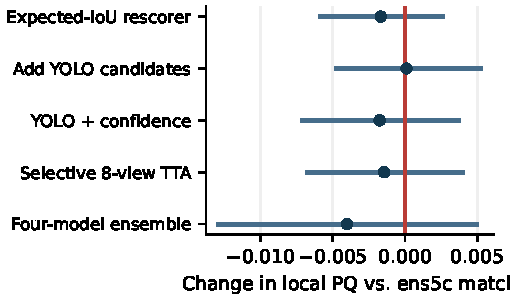
\includegraphics[width=\columnwidth]{figures/paired_comparisons.pdf}
\caption{Recorded nested-rescorer comparisons with the five-model match
baseline. Points are PQ differences; bars are paired 95\% bootstrap
intervals. These intervals are descriptive after model selection.}
\end{figure}

\subsection{What did not justify replacement}
Adding YOLO11s-seg candidates changes nested PQ by only $+0.00010$, with
95\% interval $[-0.00476,+0.00521]$. Confidence features do not improve
that result. The raw low-threshold YOLO prediction has PQ 0.34769; it is
not directly comparable to a fully filtered ensemble. Detector candidates
remain useful research evidence, but do not justify a more complex final
pipeline here. No comparable Mask R-CNN result was established, so we do
not rank an untrained architecture above a measured submission.

Eight-view test-time augmentation, nonuniform ensemble weights, larger
training crops, FPN, and additional seeds did not reliably improve the
complete pipeline. A selectively applied contour refiner raised local
PQ from 0.47404 to 0.47530, but its paired interval included zero and
its development procedure added further selection. It was not included.
Transformer experiments begun near the deadline are excluded from the
results in this report unless separately validated and documented.

\clearpage
\twocolumn[{\centering
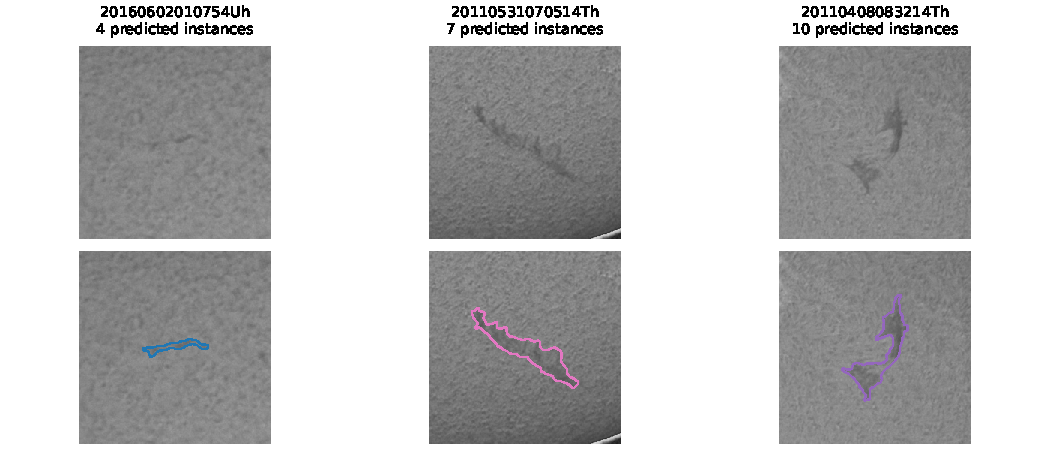
\includegraphics[width=.94\textwidth]{figures/morphology.pdf}
\captionof{figure}{Morphology examples from the accepted match submission. Top:
native-resolution image crops. Bottom: the same crops with predicted
instance contours. Observations are selected deterministically at the
25th, 50th and 75th percentiles of predicted instance count; the crop
contains the largest predicted filament. These are test-image predictions
without ground truth and illustrate morphology, not accuracy.}
\vspace{1em}}]

\section{Morphology, failure modes, and limitations}
Native-resolution prediction preserves detail. Contact regions separate
neighbors and fragment merging reconnects disconnected parts, but either
can misgroup physical structures. Global dilation, erosion, hole filling
and contour smoothing did not provide useful gains.

Small and faint filaments are an important source of missed objects.
Some apparent false positives are marked by another annotator, so plausible
morphology need not imply consistent scoring. Consensus supervision and
rescoring do not resolve that physical ambiguity. Retaining at least one
candidate per image is a submission convention that can add a false
positive on a truly empty observation, not an astronomical prior.

The split is grouped by observation, not by month or solar event, so
neighboring observations may be correlated. Test contains proportionally
more 2021--2022 images than development. Oversampling these years did not
improve validation. We do not attribute the local-to-public gap to a single
known cause. No externally task-trained solar checkpoint is included.

SQ describes only matched pairs. It does not establish one-to-many or
many-to-one physical correspondence distributions. Those diagnostics and
an independent temporal holdout remain limitations of this evaluation.

\section{Reproducibility and release contents}
The companion repository provides pinned Python dependencies, the exact
five checkpoint byte streams, both rescorers, training configurations,
logs, split IDs, and a notebook that performs fresh inference. Checkpoints
are stored as ordered chunks below standard repository file-size limits;
the restoration script checks individual and reconstructed SHA-256 hashes.
No re-training or external checkpoint download is needed for inference.
Competition images and annotation polygons are not redistributed: the
notebook expects the official dataset supplied under its access terms.

Both rescorers share one segmentation inference pass. The reference CSVs
are used only for a final agreement check, never as model inputs. On
14 November 2026, independent structural audits of the submitted files
confirmed 180 covered observations, 1,214 match-target instances and 1,221
expected-IoU instances, valid nonempty RLE, unique IDs, and zero overlapping
prediction pixels. The package records checksums and can report decoded
agreement when hardware-dependent boundary differences prevent byte-exact
reproduction. Structural validity and agreement with a submitted CSV do
not measure accuracy on hidden labels.

The implementation was developed on an 8\,GB NVIDIA RTX 5070 Laptop GPU.
Arrays are processed per observation, with one GPU job at a time.
Architecture and package authors are credited below; pretrained-model and
competition-data terms remain applicable.

\begin{thebibliography}{6}
\bibitem{challenge} NSF National Solar Observatory. Solar Filament
Segmentation Challenge 2026: data, evaluation, and final submission.
\url{https://www.kaggle.com/competitions/filament-segmentation-2026}.
\bibitem{unet} O. Ronneberger, P. Fischer, and T. Brox. 2015.
U-Net: Convolutional Networks for Biomedical Image Segmentation.
\url{https://arxiv.org/abs/1505.04597}.
\bibitem{resnet} K. He, X. Zhang, S. Ren, and J. Sun. 2015.
Deep Residual Learning for Image Recognition.
\url{https://arxiv.org/abs/1512.03385}.
\bibitem{convnext} Z. Liu et al. 2022. A ConvNet for the 2020s.
\url{https://arxiv.org/abs/2201.03545}.
\bibitem{dinov3} O. Sim\'eoni et al. 2025. DINOv3.
\url{https://arxiv.org/abs/2508.10104}.
\bibitem{smp} P. Iakubovskii and contributors. Segmentation Models PyTorch.
\url{https://github.com/qubvel-org/segmentation_models.pytorch}.
\end{thebibliography}
\end{document}
